\section{Applications of DSSAT}
\label{sect:dssat-application}

In this section, we demonstrate two applications of DSSAT.

\subsection{Analyzing probabilistic/approximate partial design}
After formulating DSSAT and proving its NEXPTIME-completeness,
we show its application to the analysis of probabilistic design and approximate design.
Specifically, we consider the probabilistic version of the \textit{topologically constrained logic synthesis problem}~\cite{Sinha2002,Balabanov2014},
or equivalently the \textit{partial design problem}~\cite{Gitina2013}.

In the \textit{(deterministic) partial design problem},
we are given a specification function $G(X)$ over primary input variables $X$ and
a \textit{partial design} $C_F$ with black boxes to be synthesized.
The Boolean functions induced at the primary outputs of $C_F$ can be described by $F(X,T)$,
where $T$ corresponds to the variables of the black box outputs.
Each black box output $t_i$ is specified with its input variables (i.e., dependency set) $\dep{i}\subseteq X \cup Y$ in $C_F$,
where $Y$ represents the variables for intermediate gates in $C_F$ referred to by the black boxes.
The partial design problem aims at deriving the black box functions $\{h_1(\dep{1}),\ldots,h_{|T|}(\dep{|T|})\}$
such that substituting $t_i$ with $h_i$ in $C_F$ makes the resultant circuit function equal $G(X)$.
The above partial design problem can be encoded as a DQBF problem;
moreover, the partial equivalence checking problem is shown to be NEXPTIME-complete~\cite{Gitina2013}.

Specifically, the DQBF that encodes the partial equivalence checking problem is of the form:
\begin{align}
    \label{eq:dssat-dqbf-partial-design}
    \forall X,\forall Y,\exists T(D).(Y \equiv E(X)) \limply (F(X,T)\equiv G(X)),
\end{align}
where $D$ consists of $(\dep{1},\ldots,\dep{|T|})$,
$E$ corresponds to the defining functions of $Y$ in $C_F$,
and the operator ``$\equiv$'' denotes element-wise equivalence between its two operands.

\begin{figure}[t]
    \centering
    \input{fig/dssat-prob-miter.tex}
    \caption{A miter for the equivalence checking of probabilistic partial design.}
    \label{fig:dssat-prob-miter}
\end{figure}

The above partial design problem can be extended to its probabilistic variant,
which is illustrated by the circuit shown in~\cref{fig:dssat-prob-miter}.
The \textit{probabilistic partial design problem} is the same as the deterministic partial design problem except that
$C_F$ is a distilled probabilistic design~\cite{LeeTC18ProbDesign} with black boxes,
whose functions at the primary outputs can be described by $F(X,Z,T)$,
where $Z$ represents the variables for the auxiliary inputs that trigger errors in $C_F$
(including the errors of the black boxes) and
$T$ corresponds to the variables of the black box outputs.
Each black box output $t_i$ is specified with its input variables (i.e., dependency set)
$\dep{i} \subseteq X \cup Y$ in $C_F$.
When $t_i$ is substituted with $h_i$ in $C_F$,
the function of the resultant circuit is required to be sufficiently close to the specification with respect to some expected probability.

\begin{theorem}
    The probabilistic partial design problem is NEXPTIME-complete.
\end{theorem}
\begin{proof}
    To show that the probabilistic partial design problem is in the NEXPTIME complexity class,
    we note that the black box functions can be guessed and validated in time exponential to the number of black box inputs.

    To show completeness in the NEXPTIME complexity class,
    we reduce the known NEXPTIME-complete DSSAT problem to the probabilistic partial design problem,
    similar to the construction used in the previous work~\cite{Gitina2013}.
    Given a DSSAT instance,
    it can be reduced to a probabilistic partial design instance in polynomial time as follows.
    Without loss of generality,
    consider the DSSAT formula~\cref{eq:dssat}.
    We create a probabilistic partial design instance by letting the specification $G$ be a tautology and
    letting $C_F$ be a probabilistic design with black boxes,
    which involves primary inputs $x_1,\ldots,x_n$ and black box outputs $y_1,\ldots,y_m$ to compute the matrix $\pf$.
    The driving inputs of the black box output $y_j$ is specified by the dependency set $\dep{y_j}$ in~\cref{eq:dssat},
    and the probability for primary input $x_i$ to evaluate to $\top$ is set to $p_i$.
    The original DSSAT formula is satisfiable with respect to a target satisfying probability $\theta$ if and only if
    there exist implementations of the black boxes such that the resultant circuit composed with the black box implementations behaves like a tautology with respect to the required expectation $\theta$.
\end{proof}

On the other hand,
the probabilistic partial design problem can be encoded with the following XDSSAT formula:
\begin{align}
    \label{eq:dssat-partial-design}
    \random{} X,\random{} Z,\forall Y,\exists T(D).(Y \equiv E(X)) \limply (F(X,Z,T)\equiv G(X)),
\end{align}
where the primary input variables are randomly quantified with probability $p_{x_i}$ of $x_i \in X$ to reflect their weights,
and the error-triggering auxiliary input variables $Z$ are randomly quantified according to the pre-specified error rates of the erroneous gates in $C_F$.
Notice that the above formula takes advantage of the extension with universal quantifiers as discussed previously.

In approximate design,
a circuit implementation may deviate from its specification by a certain extent.
The amount of deviation can be characterized in a way similar to the error probability calculation in probabilistic design.
For approximate partial design,
the equivalence checking problem can be expressed by the XDSSAT formula:
\begin{align}
    \label{eq:dssat-approximate-design}
    \random{} X,\forall Y,\exists T(D).(Y \equiv E(X)) \limply (F(X,T)\equiv G(X)),
\end{align}
which differs from~\cref{eq:dssat-partial-design} only in requiring no auxiliary inputs.
The probabilities of the randomly quantified primary input variables are determined by the approximation criteria in measuring the deviation.
For example, when all the input assignments are of equal weight,
the probabilities of the primary inputs are all set to 0.5.

We note that as the engineering change order (ECO) problem~\cite{JiangDATE20ECOSurvey} heavily relies on partial design equivalence checking,
the above DSSAT formulations provide fundamental bases for ECOs of probabilistic and approximate designs.

\subsection{Modeling Dec-POMDP}
\begin{figure*}[t]
    \centering
    \begin{tcolorbox}[colback=white]
    \begin{align}
    &\bigwedge_{0\leq t\leq h-2}[x_p^t \equiv \bot\rightarrow\bigwedge_{i\in I}x_o^{i,t} \equiv 0\wedge x_s^{t+1} \equiv 0\wedge x_p^{t+1} \equiv \bot]\label{eq:xp_next}\\
    &x_p^{h-1}\equiv\bot\label{eq:xp_stop}\\
    &\bigwedge_{s\in S}\bigwedge_{\vec{a}\in\vec{A}}[x_p^0 \equiv\bot\wedge x_s^0 \equiv s \wedge\bigwedge_{i\in I}x_a^{i,0}\equiv a_i \rightarrow x_r^0 \equiv N_r(s,\vec{a})]\label{eq:xr_0}\\
    &\bigwedge_{1\leq t\leq h-1}\bigwedge_{s\in S}\bigwedge_{\vec{a}\in\vec{A}}[x_p^{t-1}\equiv\top\wedge x_p^t \equiv\bot\wedge x_s^t \equiv s \wedge\bigwedge_{i\in I}x_a^{i,t}\equiv a_i\rightarrow
    x_r^t \equiv N_r(s,\vec{a})]\label{eq:xr_t}\\
    &\bigwedge_{0\leq t\leq h-2}\bigwedge_{s\in S}\bigwedge_{\vec{a}\in\vec{A}}\bigwedge_{s'\in S}[x_p^t \equiv \top\wedge x_s^t \equiv s \wedge\bigwedge_{i\in I}x_a^{i,t}\equiv a_i\wedge x_s^{t+1}\equiv s'\rightarrow x_{T_{s,\vec{a}}}^t \equiv s']\label{eq:x_T}\\
    &\bigwedge_{0\leq t\leq h-2}\bigwedge_{s'\in S}\bigwedge_{\vec{a}\in\vec{A}}\bigwedge_{\vec{o}\in\vec{O}}[x_p^t \equiv\top\wedge x_s^{t+1} \equiv s'\wedge\bigwedge_{i\in I}x_a^{i,t}\equiv a_i\wedge\bigwedge_{i\in I}x_o^{i,t}\equiv o_i\rightarrow x_{\Omega_{s',\vec{a}}}^t \equiv N_\Omega(\vec{o})]\label{eq:x_omega}
\end{align}
\end{tcolorbox}
    \caption{The formulas used to encode a Dec-POMDP $\mathcal{M}$.}\label{fig:formula}
    \vspace{-0.5cm}
\end{figure*}

In this section we demonstrate the descriptive power of DSSAT to model NEXPTIME-complete problems by constructing a polynomial-time reduction from Dec-POMDP to DSSAT.
Our reduction is an extension of that from POMDP to SSAT proposed in the previous work~\cite{Salmon2020}.

In essence, given a Dec-POMDP $\mathcal{M}$, we will construct in polynomial time a DSSAT formula $\Phi$ such that there is a joint policy $\vec{\pi}$ for $\mathcal{M}$ with value $V(\vec{\pi})$ if and only if there is a set of Skolem functions $\mathcal{F}$ for $\Phi$ with satisfying probability $\Pr[\Phi|_{\mathcal{F}}]$, and $V(\vec{\pi})=\Pr[\Phi|_{\mathcal{F}}]$.

First we introduce the variables used in construction of the DSSAT formula and their domains.
To improve readability, we allow a variable $x$ to take values from a finite set $U=\{x_1,\ldots,x_K\}$~\cite{Salmon2020}.
Under this setting, a randomized quantifier $\random{}$ over variable $x$ specifies a distribution $\Pr[x\equiv x_i]$ for each $x_i\in U$.
We also define a scaled reward function:
\[
    r(s,\vec{a})=\frac{\rho(s,\vec{a})-\min_{s',\vec{a}'}\rho(s',\vec{a}')}{\sum_{s'',\vec{a}''}[\rho(s'',\vec{a}'')-\min_{s',\vec{a}'}\rho(s',\vec{a}')]}
\]
such that $r(s,\vec{a})$ forms a distribution over all pairs of $s$ and $\vec{a}$, i.e., $\forall s,\vec{a}.r(s,\vec{a})\geq 0$ and $\sum_{s,\vec{a}}r(s,\vec{a})=1$.
We will use the following variables:
\begin{itemize}
    \item $x_s^t\in S$: the state at stage $t$,
    \item $x_a^{i,t}\in A_i$: the action taken by Agent $i$ at stage $t$,
    \item $x_o^{i,t}\in O_i$: the observation received by Agent $i$ at stage $t$,
    \item $x_r^t\in S\times (A_1\times\ldots\times A_n)$: the reward earned at stage $t$,
    \item $x_T^t\in S$: transition distribution at stage $t$,
    \item $x_\Omega^t\in O_1\times\ldots\times O_n$: observation distribution at stage $t$,
    \item $x_p^t\in \mathbb{B}$: used to sum up rewards across stages.
\end{itemize}

\begin{figure*}[t]
    \centering
    \input{fig/derivation}
    \caption{The derivation of the induction case in the proof of Theorem~\ref{thm:reduction}.}
    \label{fig:derivation}
\end{figure*}

We represent elements in the sets $S$, $A_i$, and $O_i$ by integers, i.e., $S=\{0,1,\ldots,|S|-1\}$, etc., and use indices $s$, $a_i$, and $o_i$ to iterate through them, respectively.
On the other hand, a special treatment is required for variables $x_r^t$ and $x_\Omega^t$, as they range over Cartesian products of several sets.
We will give a unique number to an element in a product set as follows.
Consider $\vec{Q}=Q_1\times\ldots\times Q_n$, where each $Q_i$ is a finite set.
An element $\vec{q}=(q_1,\ldots,q_n)\in \vec{Q}$ is numbered by $N(q_1,\ldots,q_n)=\sum_{i=1}^n q_i(\prod_{j=1}^{i-1}|Q_j|)$.
In the following construction, variables $x_r^t$ and $x_\Omega^t$ will take values from the numbers given to the elements in $S\times\vec{A}$ and $\vec{O}$ by $N_r(s,\vec{a})$ and $N_\Omega(\vec{o})$, respectively.

We begin by constructing a DSSAT formula for a Dec-POMDP with $h=1$.
Under this setting, the derivation of the optimal joint policy is simplified to finding an action for each agent such that the expectation value of the reward function is maximized, i.e.,
\[
    \vec{a}^*=\argmax_{\vec{a}\in \vec{A}}\sum_{s\in S}\Delta_0(s)r(s,\vec{a})
\]
The DSSAT formula below encodes the above equation:
\[
    \random{} x_s^0,\random{} x_r^0,\exists x_a^{1,0}(D_{x_a^{1,0}}),\ldots,\exists x_a^{n,0}(D_{x_a^{n,0}}).\phi,
\]
where the distribution of $x_s^0$ follows $\Pr[x_s^0 \equiv s]=\Delta_0(s)$, the distribution of $x_r^0$ follows $\Pr[x_r^0 \equiv N_r(s,\vec{a})]=r(s,\vec{a})$, each $D_{x_a^{i,0}}=\emptyset$, and the matrix:
\[
    \phi=\bigwedge_{s\in S}\bigwedge_{\vec{a}\in\vec{A}}[x_s^0\equiv s\wedge\bigwedge_{i\in I} x_a^{i,0}\equiv a_i\rightarrow x_r^0\equiv N_r(s,\vec{a})].
\]
As the existentially quantified variables have no dependency on randomly quantified variable, the DSSAT formula is effectively an exist-random quantified SSAT formula.

For an arbitrary Dec-POMDP with $h>1$, we follow the two steps proposed in the previous work~\cite{Salmon2020}, namely \textit{policy selection} and \textit{policy evaluation}, and adapt the policy selection step for the multi-agent setting in Dec-POMDP.

In the previous work~\cite{Salmon2020}, an agent's policy selection is encoded by the following prefix (use Agent $i$ as an example):
\[
    %\exists x_a^{i,0},\random{} x_p^0,\random{} x_o^{i,0},\ldots,\exists x_a^{i,h-2},\random{} x_p^{h-2},\random{} x_o^{i,h-2},\exists x_a^{i,h-1},\random{} x_p^{h-1}.
    \exists x_a^{i,0},\random{} x_p^0,\random{} x_o^{i,0},\ldots,\random{} x_p^{h-2},\random{} x_o^{i,h-2},\exists x_a^{i,h-1},\random{} x_p^{h-1}.
\]
In the above quantification, variable $x_p^t$ is introduced to sum up rewards earned at different stages.
It takes values from $\mathbb{B}$, and follows a uniform distribution, i.e., $\Pr[x_p^t \equiv \top]=\Pr[x_p^t \equiv \bot]=0.5$.
When $x_p^t \equiv \bot$, the process is stopped and the reward at stage $t$ is earned; when $x_p^t \equiv \top$, the process is continued to stage $t+1$.
Note that variables $\{x_p^t\}$ are shared across all agents.
With the help of variable $x_p^t$, rewards earned at different stages are summed up with an equal weight $2^{-h}$.
Variable $x_o^{i,t}$ also follows a uniform distribution $\Pr[x_o^{i,t} \equiv o_i]=|O_i|^{-1}$, which scales the satisfying probability by $|O_i|^{-1}$ at each stage.
Therefore, we need to re-scale the satisfying probability accordingly in order to obtain the correct satisfying probability corresponding to the value of a joint policy.
The scaling factor will be derived in the proof of Theorem~\ref{thm:reduction}.

As the actions of the agents can only depend on their own observation history, for the selection of a joint policy it is not obvious how to combine the quantification, i.e., the selection of a policy, of each agent into a linearly ordered prefix required by SSAT, without suffering an exponential translation cost.
On the other hand, DSSAT allows to specify the dependency of an existentially quantified variable freely and is suitable to encode the selection of a joint policy.
In the prefix of the DSSAT formula, variable $x_a^{i,t}$ depends on $D_{x_a^{i,t}}=\{x_o^{i,0},\ldots,x_o^{i,t-1},x_p^0,\ldots,x_p^{t-1}\}$.

Next, the policy evaluation step is exactly the same as that in the previous work~\cite{Salmon2020}.
The following quantification computes the value of a joint policy:
\begin{align*}
    \random{} x_s^t, \random{} x_r^t, t=0,\ldots,h-1 \\
    \random{} x_T^t, \random{} x_\Omega^t, t=0,\ldots,h-2
\end{align*}
Variables $x_s^t$ follow a uniform distribution $\Pr[x_s^t \equiv s]=|S|^{-1}$ except for variable $x_s^0$, which follows the initial distribution specified by $\Pr[x_s^0 \equiv s]=\Delta_0(s)$; variables $x_r^t$ follow the distribution of the reward function $\Pr[x_r^t \equiv N_r(s,\vec{a})]=r(s,\vec{a})$; variables $x_T^t$ follow the state transition distribution $\Pr[x_{T_{s,\vec{a}}}^t \equiv s']=T(s,\vec{a},s')$; variables $x_\Omega^t$ follow the observation distribution $\Pr[x_{\Omega_{s',\vec{a}}}^t \equiv N_\Omega(\vec{o})]=\Omega(s',\vec{a},\vec{o})$.
Note that these variables encode the random mechanism of a Dec-POMDP and are hidden from agents.
That is, variables $x_a^{i,t}$ do not depend on the above variables.

\begin{figure*}[t]
    \centering
    \begin{tikzpicture}
  \begin{scope}
    \Tree [.$\exists x_a^{1,0}x_a^{2,0}$
    \edge node[auto=right]{$\vec{a}^0=(a_1^0,a_2^0)$}; [.${\random{}x_p^0}$
    \edge node[auto=right]{0.5}; [.${\random{}x_o^{1,0},\random{}x_o^{2,0}}$
    \edge node[auto=right]{$\frac{1}{|O_1\times O_2|}$}; [.$\exists x_a^{1,1}x_a^{2,1}$
    [.${\random{} x_p^1}$
    \edge node[auto=right]{0.5}; [.${\random{}x_s,\random{}x_r,\random{}x_T,\random{}x_\Omega}$
    \edge node[auto=right]{$\frac{1}{|S|}$}; [.$\Delta_0(s^0)r(s^0,\vec{a}^0)$ ]
    [.... ]
    [.... ]
    [.... ]
    [.... ] ]
    \edge node[auto=left]{0.5}; [.$0$ ] ] ]
    [.$0\cdots$ ]
    [.$\cdots 0$ ] ]
    \edge node[auto=left]{0.5}; [.${\random{}x_o^{1,0},\random{}x_o^{2,0}}$
    \edge node[auto=right]{$\frac{1}{|O_1\times O_2|}$}; [.$\exists x_a^{1,1}x_a^{2,1}$ ]
    [.... ]
    \edge node[auto=left]{$\vec{o}^0=(o_1^0,o_2^0)$}; [.$\exists x_a^{1,1}x_a^{2,1}$
    \edge node[auto=right]{$\vec{a}^1=(a_1^1,a_2^1)$}; [.${\random{}x_p^1}$
    \edge node[auto=right]{0.5}; [.${\random{}x_s,\random{}x_r,\random{}x_T,\random{}x_\Omega}$
    \edge node[auto=right]{$\frac{1}{|S|}$}; [.$\Delta_0(s^0)T(s^0,\vec{a}^0,s^1)\Omega(s^1,\vec{a}^0,\vec{o}^0)r(s^1,\vec{a}^1)$ ]
    [.... ]
    [.... ] ]
    \edge node[auto=left]{0.5}; [.$0$ ] ] ] ] ] ]
  \end{scope}
\end{tikzpicture}
    \caption{The decision tree of a Dec-POMDP example with two agents and $h=2$.}
    \label{fig:example}
    \vspace{-0.5cm}
\end{figure*}

The formulas to encode $\mathcal{M}$ are listed in Figure~\ref{fig:formula}.
Formula~\eqref{eq:xp_next} encodes that when $x_p^t \equiv \bot$, i.e., the process is stopped, the observation $x_o^{i,t}$ and next state $x_s^{t+1}$ are set to a preserved value $0$, and $x_p^{t+1} \equiv \bot$.
Formula~\eqref{eq:xp_stop} ensures the process is stopped at the last stage.
Formula~\eqref{eq:xr_0} ensures the reward at the first stage is earned when the process is stopped, i.e., $x_p^0 \equiv \bot$.
Formula~\eqref{eq:xr_t} requires the reward at stage $t>0$ is earned when $x_p^{t-1} \equiv \top$ and $x_p^t \equiv \bot$.
Formula~\eqref{eq:x_T} encodes the transition distribution from state $s$ to state $s'$ given actions $\vec{a}$ are taken.
Formula~\eqref{eq:x_omega} encodes the observation distribution to receive observation $\vec{o}$ under the situation that state $s'$ is reached after actions $\vec{a}$ are taken.

\begin{theorem}\label{thm:reduction}
    The above reduction maps a Dec-POMDP $\mathcal{M}$ to a DSSAT formula $\Phi$, such that a joint policy $\vec{\pi}$ exists for $\mathcal{M}$ if and only if a set of Skolem functions $\mathcal{F}$ exists for $\Phi$, with $V(\vec{\pi})=\Pr[\Phi|_{\mathcal{F}}]$.
\end{theorem}
\begin{proof}
    Given an arbitrary Dec-POMDP $\mathcal{M}$, a proof using mathematical induction over its planning horizon $h$ is as follows.

    For the base case $h=1$, to prove the ``only if'' direction, consider a joint policy $\vec{\pi}$ for $\mathcal{M}$ which specifies $\vec{a}=(a_1,\ldots,a_n)$ where agent $i$ will take action $a_i$. For this joint policy, the value is computed as $V(\vec{\pi})=\sum_{s \in S}\Delta_0(s)r(s,\vec{a})$. Based on $\vec{\pi}$, we construct a set of Skolem functions $\mathcal{F}$ where $x_a^{i,0}=a_i$ for each $i\in I$. To compute $\Pr[\Phi|_{\mathcal{F}}]$, we cofactor the matrix with $\mathcal{F}$ and arrive at the following CNF formula:
    \[
        \bigwedge_{s\in S}[x_s^0\neq s \vee x_r^0 \equiv N_r(s,\vec{a})],
    \]
    and the satisfying probability of $\Phi$ with respect to $\mathcal{F}$ is
    \begin{align*}
        \Pr[\Phi|_{\mathcal{F}}] & =\sum_{s\in S}\Pr[x_s^0 \equiv s]\Pr[x_r^0 \equiv N_r(s,\vec{a})] \\
                                 & =\sum_{s\in S}\Delta_0(s)r(s,\vec{a})=V(\vec{\pi})
    \end{align*}

    Note in the above argument, only equalities are involved, and hence can be reversed to prove the ``if'' direction.

    For the induction case $h>1$, first assume that the statement holds. For a planning horizon of $h+1$, consider a joint policy $\vec{\pi}_{h+1}$ with value $V(\vec{\pi}_{h+1})$. Note that as a joint policy is a mapping from observation histories to actions, we can build a corresponding set of Skolem functions $\mathcal{F}_{h+1}$ to simulate joint policy $\vec{\pi}_{h+1}$ for the DSSAT formula. The derivation of satisfying probability with respect to $\mathcal{F}_{h+1}$ is shown in Figure~\ref{fig:derivation}. Note that to obtain the correct value of the joint policy, we need to re-scale the satisfying probability by a scaling factor $\kappa_{h+1}=2^{h+1}(|\vec{O}||S|)^{h}$.

    Once again, as only equalities are involved in the derivation in Figure~\ref{fig:derivation}, the ``if'' direction is also proved.

    As $\Pr[\Phi|_{\mathcal{F}_{h+1}}]=V(\vec{\pi}_{h+1})$, the theorem is proved according to the principle of mathematical induction.
\end{proof}

\subsection{Discussion}
Below we count the numbers of variables and clauses in the resulting DSSAT formula with respect to the input size of the given Dec-POMDP.
For one stage, there are $3+2(|I|+|S||\vec{A}|)$ variables, and therefore in total the number of variables is $O(h(|I|+|S||A|))$ asymptotically.
On the other hand, the number of clauses per stage is $2+|I|+|S||\vec{A}|+|S|^2|\vec{A}|+|S||\vec{A}||\vec{O}|$, and hence the total number of clauses is $O(h(|I|+|S||\vec{A}|(|S|+|\vec{O}|))$.
Overall, we show that the proposed reduction is polynomial-time with respect to the input size of the Dec-POMDP.

Below we demonstrate the reduction with an example.

\begin{example}
    Consider a Dec-POMDP with two agents and planning horizon $h=2$.
    Given a joint policy $(\pi_1,\pi_2)$ for Agent $1$ and Agent $2$, let the actions taken at $t=0$ be $\vec{a}^0=(a_1^0,a_2^0)$ and the actions taken at $t=1$ under certain observations $\vec{o}^0=(o_1^0,o_2^0)$ be $\vec{a}^1=(a_1^1,a_2^1)$.
    The value of this joint policy is computed by~\cref{eq:dssat-bellman} as
    \begin{align*}
        V(\pi) & =\sum_{s^0\in S}\Delta_0(s^0)[r(s^0,\vec{a}^0)                                                                  \\
               & +\sum_{\vec{o}^0\in\vec{O}}\sum_{s^1\in S}T(s^0,\vec{a}^0,s^1)\Omega(s^1,\vec{a}^0,\vec{o}^0)r(s^1,\vec{a}^1)].
    \end{align*}

    The decision tree of the converted DSSAT formula is shown in Figure~\ref{fig:example}.
    At $t=0$, after taking actions $\vec{a}^0$, variable $x_p^0$ splits into two cases: when $x_p^0\equiv \bot$ (left branch), the expected reward $\Delta_0(s^0)r(s^0,\vec{a}^0)$ will be earned for $t=0$; on the other hand, when $x_p^0\equiv \top$ (right branch), observation $\vec{o}^0$ is received, based on which the agents will select their actions $\vec{a}^1$ at $t=1$.
    Again, variable $x_p^1$ will split into two cases, but this time $x_p^1$ is forced to be $\bot$ as it is the last stage.
    The expected reward $\Delta_0(s^0)T(s^0,\vec{a}^0,s^1)\Omega(s^1,\vec{a}^0,\vec{o}^0)r(s^1,\vec{a}^1)$ will be earned under the branch of $x_p^1\equiv\bot$ for $t=1$.
    Note that the randomized quantifiers over variables $x_p^t$, $x_s^t$, and $x_o^t$ will scale the satisfying probability by the factors labelled on the edges, respectively.
    Therefore, we have to re-scale the satisfying probability by $2^2|S||O_1\times O_2|$, which is predicted by the scaling factor $\kappa_{h}=2^h(|\vec{O}||S|)^{h-1}$ calculated in the proof of Theorem~\ref{thm:reduction}.
\end{example}